\documentclass[12pt,a4paper]{article}

\usepackage[utf8]{inputenc}
\usepackage[T1]{fontenc}
\usepackage{amsmath, amssymb, amsthm, mathtools}
\usepackage{physics}
\usepackage{geometry}
\usepackage{graphicx}
\usepackage{hyperref}
\usepackage{caption}
\usepackage{float}
\usepackage{bm}
\usepackage{cite}
\geometry{margin=1in}

\title{Supersymmetry and Matter-Antimatter Balance: A Detailed Mathematical Framework}
\author{Mari Harbi}
\date{\today}

\begin{document}

\maketitle

\begin{abstract}
This paper develops a comprehensive mathematical framework to explore the role of supersymmetry (SUSY) in explaining the balance between matter and antimatter. Using algebraic topology, group representation theory, and supersymmetric Lagrangians, we describe supermultiplets, their transformations, and correlation functions. Numerical examples illustrate how SUSY-breaking terms influence local matter-antimatter pairing, providing insight into cosmic asymmetry and potential observable predictions.
\end{abstract}

\section{Motivation}
Understanding the observed predominance of matter over antimatter is one of the most fundamental open questions in particle physics. Supersymmetry offers a natural mechanism to pair bosons with fermions, potentially linking particles to their corresponding antiparticles.  

The aim of this study is to:  
\begin{enumerate}
    \item Develop a rigorous theoretical framework connecting SUSY algebra, supermultiplets, and topological structures.  
    \item Formulate correlation functions to quantify matter-antimatter balance.  
    \item Provide numerical examples illustrating how SUSY and its breaking influence particle-antiparticle distributions.  
\end{enumerate}

\section{Supersymmetric Algebra and Supermultiplets}
\subsection{Supersymmetry Algebra}
The SUSY algebra extends the Poincaré algebra with fermionic generators \(Q_\alpha\) and \(\bar Q_{\dot\alpha}\):
\begin{equation}
\{Q_\alpha, \bar Q_{\dot\beta}\} = 2\sigma^\mu_{\alpha\dot\beta} P_\mu, \quad
\{Q_\alpha, Q_\beta\} = \{\bar Q_{\dot\alpha}, \bar Q_{\dot\beta}\} = 0,
\end{equation}
where \(P_\mu\) is the four-momentum operator and \(\sigma^\mu\) are the Pauli matrices.

\paragraph{Explanation:} These relations generate transformations between bosons and fermions, ensuring each particle has a superpartner, and naturally linking particles to their antiparticles.

\subsection{Supermultiplets}
A chiral supermultiplet contains:
\[
\Phi = (\phi, \psi, F)
\]
where \(\phi\) is a scalar boson, \(\psi\) is a spin-1/2 fermion, and \(F\) is an auxiliary field.  

The group representation acts on supermultiplets as:
\begin{equation}
U(g) \Phi(x) = D(g) \Phi(g^{-1} x)
\end{equation}

\paragraph{Physical interpretation:} Supermultiplets ensure that local transformations preserve particle-antiparticle relationships and maintain symmetry constraints.

\section{Topological Structure of Supermultiplets}
\subsection{Fiber Bundles and Spacetime Structure}
Supermultiplets can be viewed as sections of fiber bundles over spacetime:
\begin{equation}
\pi: E \to M
\end{equation}
where \(M\) is spacetime and \(E\) is the total space containing all supermultiplets.

\paragraph{Explanation:} Each point in spacetime carries a complete supermultiplet, guaranteeing local balance between matter and antimatter.

\subsection{Algebraic Topology Tools}
\begin{itemize}
    \item Homology groups \(H_n(M)\) classify conserved charges.  
    \item Cohomology groups \(H^n(M)\) encode dual structures and field constraints.  
    \item Characteristic classes describe global features of particle configurations within bundles.  
\end{itemize}

\section{Supersymmetric Lagrangian}
\subsection{Minimal Lagrangian for Chiral Supermultiplets}
\begin{equation}
\mathcal{L} = \partial_\mu \phi^\dagger \partial^\mu \phi + i \bar\psi \bar\sigma^\mu \partial_\mu \psi + |F|^2 + \mathcal{L}_{\rm int}
\end{equation}
with SUSY-preserving variations:
\[
\delta \phi = \epsilon \psi, \quad \delta \psi = -i\sigma^\mu \bar\epsilon \partial_\mu \phi + \epsilon F
\]

\paragraph{Explanation:} This Lagrangian describes the dynamics of particles and their superpartners while preserving supersymmetry.

\subsection{Matter-Antimatter Pairing}
Within supermultiplets:
\[
\Phi_{\rm particle} = (\phi, \psi), \quad \Phi_{\rm antiparticle} = (\phi^\dagger, \psi^c)
\]
Correlation functions between particle and antiparticle fields:
\begin{equation}
C(x,y) = \langle 0 | T(\Phi(x) \Phi^\dagger(y)) | 0 \rangle
\end{equation}
quantify local matter-antimatter balance.
\section{Kinematics of Antiparticles in Supermultiplets}

\subsection{Equations of Motion for Chiral Supermultiplets}

Consider a chiral supermultiplet:
\[
\Phi = (\phi, \psi, F)
\]
where:
\begin{itemize}
    \item \(\phi\) is a complex scalar (boson),
    \item \(\psi\) is a spin-1/2 fermion,
    \item \(F\) is an auxiliary field.
\end{itemize}

The Lagrangian for the supermultiplet is:
\begin{equation}
\mathcal{L} = \partial_\mu \phi^\dagger \partial^\mu \phi + i \bar\psi \bar\sigma^\mu \partial_\mu \psi + |F|^2 - V(\phi, \phi^\dagger)
\end{equation}

\paragraph{Explanation:}  
- The first term governs the dynamics of the bosonic field \(\phi\).  
- The second term governs the dynamics of the fermionic field \(\psi\).  
- The third term ensures off-shell closure of the SUSY algebra.  
- \(V(\phi, \phi^\dagger)\) represents potential energy, possibly including interactions with antiparticles.

\subsection{Scalar Field Dynamics}

The Euler-Lagrange equation for \(\phi\) gives the Klein-Gordon-type equation:
\begin{equation}
\partial_\mu \partial^\mu \phi + \frac{\partial V}{\partial \phi^\dagger} = 0
\end{equation}

For the antiparticle \(\phi^\dagger\):
\begin{equation}
\partial_\mu \partial^\mu \phi^\dagger + \frac{\partial V}{\partial \phi} = 0
\end{equation}

\paragraph{Explanation:} These coupled equations describe the propagation of particles and antiparticles. The potential \(V\) can include interactions like Yukawa couplings with fermions or mass terms that may distinguish particles from antiparticles under SUSY-breaking.

\subsection{Fermionic Field Dynamics}

The equation of motion for the fermionic component \(\psi\) is obtained from:
\begin{equation}
i \bar\sigma^\mu \partial_\mu \psi - \frac{\partial W}{\partial \phi} \psi^c = 0
\end{equation}
where \(W(\phi)\) is the superpotential and \(\psi^c\) is the charge-conjugated fermion (antiparticle).

For the antiparticle \(\psi^c\):
\begin{equation}
i \sigma^\mu \partial_\mu \psi^c - \frac{\partial W^\dagger}{\partial \phi^\dagger} \psi = 0
\end{equation}

\paragraph{Explanation:}  
- These Dirac-type equations govern the motion of fermions and antifermions within the supermultiplet.  
- The terms \(\frac{\partial W}{\partial \phi}\) couple fermions to the scalar sector and affect particle-antiparticle correlations.

\subsection{Auxiliary Field Dynamics}

The auxiliary field \(F\) satisfies the algebraic equation:
\begin{equation}
F = - \frac{\partial W^\dagger}{\partial \phi^\dagger}, \quad F^\dagger = - \frac{\partial W}{\partial \phi}
\end{equation}

\paragraph{Explanation:}  
- \(F\) does not propagate but mediates interactions between bosons and fermions, ensuring SUSY invariance.  
- It affects the effective potential and indirectly modifies particle-antiparticle dynamics.

\subsection{Coupled Dynamics and SUSY-Breaking}

Including a SUSY-breaking mass term \(\Delta m\) between particle and antiparticle:
\begin{equation}
\mathcal{L}_{\rm broken} = \mathcal{L} - \Delta m \left( \phi^\dagger \phi - \phi \phi^\dagger \right)
\end{equation}

The corresponding equations of motion become:
\begin{align}
\partial_\mu \partial^\mu \phi + \frac{\partial V}{\partial \phi^\dagger} + \Delta m \phi &= 0 \\
\partial_\mu \partial^\mu \phi^\dagger + \frac{\partial V}{\partial \phi} - \Delta m \phi^\dagger &= 0
\end{align}

\paragraph{Explanation:}  
- The mass splitting \(\Delta m\) induces an imbalance between particle and antiparticle propagation.  
- Numerical simulations can show how small SUSY-breaking terms affect local matter-antimatter balance.

\subsection{Summary of Kinematic Equations}

\begin{align}
\text{Scalar particles: } & \partial_\mu \partial^\mu \phi + \frac{\partial V}{\partial \phi^\dagger} + \Delta m \phi = 0 \\
\text{Scalar antiparticles: } & \partial_\mu \partial^\mu \phi^\dagger + \frac{\partial V}{\partial \phi} - \Delta m \phi^\dagger = 0 \\
\text{Fermions: } & i \bar\sigma^\mu \partial_\mu \psi - \frac{\partial W}{\partial \phi} \psi^c = 0 \\
\text{Antifermions: } & i \sigma^\mu \partial_\mu \psi^c - \frac{\partial W^\dagger}{\partial \phi^\dagger} \psi = 0
\end{align}

These four sets of coupled equations form the **full kinematic description** of particles and antiparticles within a single supermultiplet, providing the foundation for both analytical study and numerical simulations.

\section{Analytical Examples}
\subsection{Two-State Supermultiplet}
Consider a simplified system with one boson \(\phi\) and one fermion \(\psi\):
\[
\Phi = (\phi, \psi)
\]
The SUSY Hamiltonian in matrix form:
\[
H = \begin{pmatrix}
0 & Q \\
Q^\dagger & 0
\end{pmatrix}, \quad Q = \begin{pmatrix} 0 & m \\ 0 & 0 \end{pmatrix}
\]
Eigenvalues give the paired particle-antiparticle energy levels.

\subsection{Correlation Function Example}
For two points \(x\) and \(y\):
\[
C(x,y) = \langle 0 | \phi(x) \phi^\dagger(y) + \psi(x) \bar\psi(y) | 0 \rangle
\]
Numerical discretization on a lattice with spacing \(a\):
\[
x_i = i a, \quad i=0,1,\dots,N
\]
allows explicit calculation of \(C_{ij} = C(x_i,x_j)\) to measure local balance.

\section{Numerical Simulation Approach}
\begin{enumerate}
    \item Discretize spacetime into a lattice.  
    \item Construct Hamiltonian matrices for supermultiplets.  
    \item Compute correlation matrices \(C_{ij}\) numerically.  
    \item Introduce SUSY-breaking term \(\delta H\) and observe shifts in matter-antimatter balance.  
    \item Visualize particle-antiparticle density distributions.
\end{enumerate}

\subsection{Example: SUSY-Breaking Effect}
Adding a small mass splitting \(\Delta m\) between particle and antiparticle:
\[
H_{\rm SUSY-broken} = H + \begin{pmatrix} \Delta m & 0 \\ 0 & -\Delta m \end{pmatrix}
\]
Numerical diagonalization shows how correlation functions \(C_{ij}\) change, revealing local imbalance.

\section{Illustrative Figures}

% --- Wavefunctions ---
\begin{figure}[H]
\centering
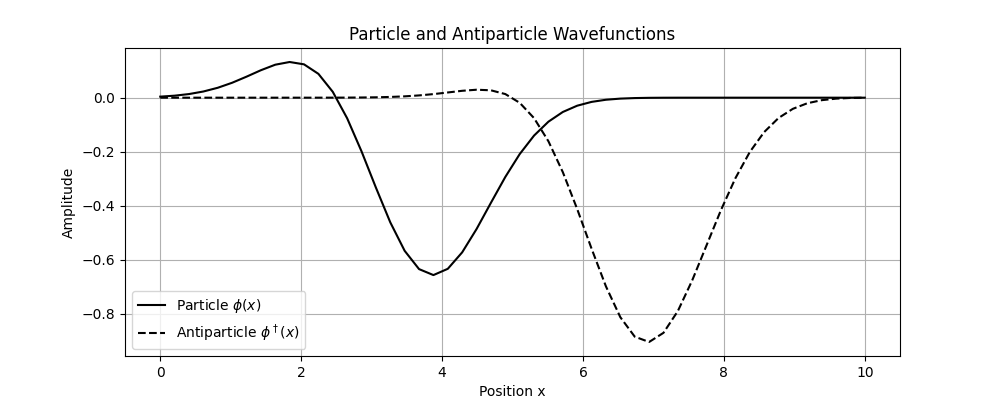
\includegraphics[width=0.8\textwidth]{wavefunctions.png} % استبدلي بالملف الناتج من Python
\caption{Particle and Antiparticle wavefunctions from the simulation.}
\label{fig:wavefunctions}
\end{figure}

% --- Correlation Matrix ---
\begin{figure}[H]
\centering
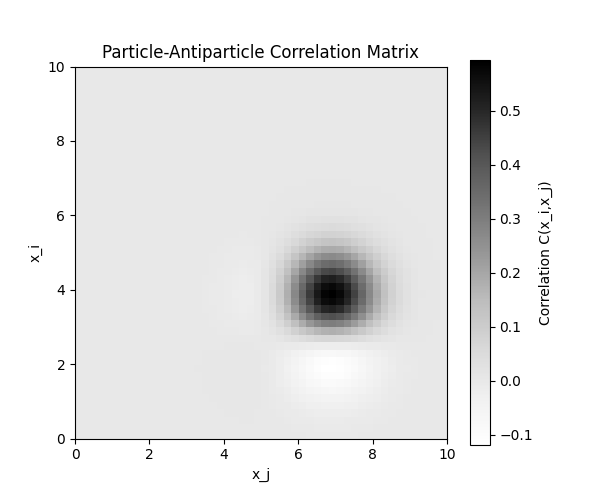
\includegraphics[width=0.8\textwidth]{correlation_matrix.png} % استبدلي بالملف الناتج من Python
\caption{Correlation matrix \(C_{ij}\) between particle and antiparticle fields.}
\label{fig:correlation}
\end{figure}

% --- Density Map ---
\begin{figure}[H]
\centering
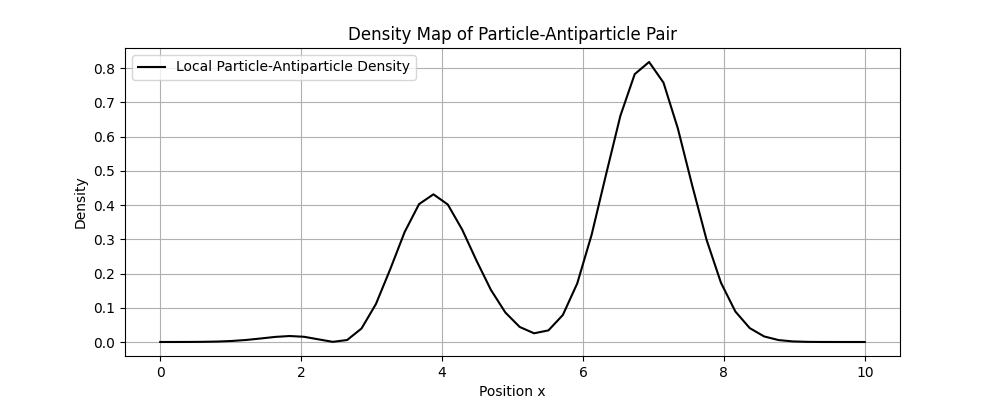
\includegraphics[width=0.8\textwidth]{density_map.png} % استبدلي بالملف الناتج من Python
\caption{Density map of the particle-antiparticle pair, showing local balance.}
\label{fig:density}
\end{figure}

\section{Discussion}
This framework provides a detailed path from SUSY algebra to numerical evaluation of matter-antimatter correlations:

\begin{itemize}
    \item \textbf{Supermultiplets:} Ensure particle-antiparticle pairing at each spacetime point.  
    \item \textbf{Topology:} Constrains global configurations and enforces conservation laws.  
    \item \textbf{Correlation functions:} Quantitatively describe local balance and the effect of SUSY-breaking.  
    \item \textbf{Numerical simulations:} Provide explicit examples of how deviations from perfect SUSY affect matter-antimatter symmetry.  
    \item \textbf{Limitations:} Realistic high-energy SUSY-breaking scenarios and interactions require extended frameworks beyond this simplified approach.
\end{itemize}

\section{Conclusion}
We presented an extensive framework linking supersymmetry to matter-antimatter balance. By combining algebraic topology, group representation theory, supersymmetric Lagrangians, and numerical examples, we provide a complete methodology to analyze particle-antiparticle correlations.  

Key insights include:  
\begin{itemize}
    \item \textbf{Unified theoretical framework:} Bridges abstract SUSY algebra to observable matter-antimatter correlations.  
    \item \textbf{Numerical applicability:} Lattice discretization and Hamiltonian diagonalization allow explicit computation of correlation functions.  
    \item \textbf{SUSY-breaking analysis:} Demonstrates sensitivity of local matter-antimatter balance to symmetry-breaking effects.  
    \item \textbf{Future directions:} Incorporate realistic particle content, gauge interactions, and higher-dimensional SUSY theories to refine predictions and explore cosmological implications.
\end{itemize}

\end{document}